\documentclass{standalone}

\usepackage{xcolor}
\usepackage{graphicx}
\usepackage{tikz}

\usetikzlibrary{shapes.geometric, arrows}
\usetikzlibrary{calc,positioning}

\graphicspath{{../../}}

\begin{document}
\nopagecolor
\large
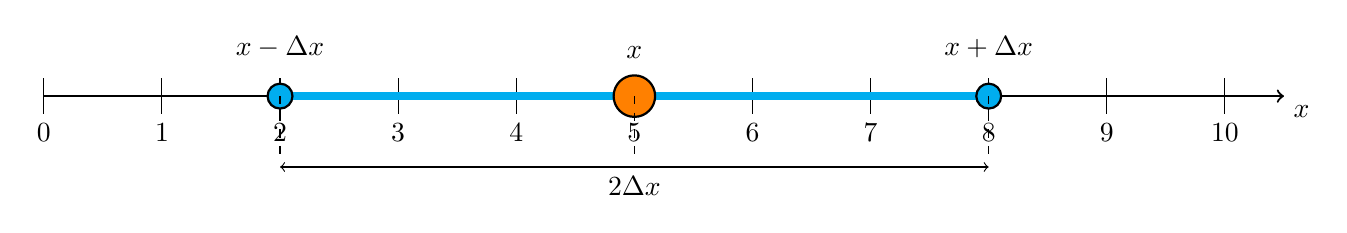
\begin{tikzpicture}[scale=1.5]

    % As
    \draw[->, thick] (0,0) -- (10.5,0);
    \node[below right] at (10.5,0) {$x$};

    % Ticks
    \foreach \x in {0,1,2,3,4,5,6,7,8,9,10} {
        \draw (\x,-0.15) -- (\x,0.15);
        \node[below] at (\x,-0.15) {\x};
    }

    \draw[line width=3pt, cyan] (2,0) -- (8,0);

    \draw[fill=cyan, thick] (2,0) circle (3pt)
        node [above=1em] {$x - \Delta x$};
    \draw[fill=cyan, thick] (8,0) circle (3pt)
        node [above=1em] {$x + \Delta x$};

    \draw[fill=orange, thick] (5,0) circle (5pt)
        node [above=1em] {$x$};

    \draw[<->] (2,-0.6) -- (8,-0.6)
        node[midway, below] {$2\Delta x$};

    \draw[dashed] (2,0) -- (2,-0.5);
    \draw[dashed] (5,0) -- (5,-0.5);
    \draw[dashed] (8,0) -- (8,-0.5);

\end{tikzpicture}
\end{document}
